\documentclass[11pt]{article}
\usepackage[sc]{mathpazo} %Like Palatino with extensive math support
\usepackage{fullpage}
\usepackage[authoryear,sectionbib,sort]{natbib}
\linespread{1.7}
\usepackage[utf8]{inputenc}
\usepackage{lineno}
\usepackage{titlesec}
% Added later
\usepackage{amsmath}  % for equations
\usepackage{graphicx} % for figures
\titleformat{\section}[block]{\Large\bfseries\filcenter}{\thesection}{1em}{}
\titleformat{\subsection}[block]{\Large\itshape\filcenter}{\thesubsection}{1em}{}
\titleformat{\subsubsection}[block]{\large\itshape}{\thesubsubsection}{1em}{}
\titleformat{\paragraph}[runin]{\itshape}{\theparagraph}{1em}{}[. ]\renewcommand{\refname}{Literature Cited}

\usepackage{color}

\usepackage{hyperref}
\definecolor{darkgreen}{rgb}{0.1,0.6,0.3}
\definecolor{darkred}{rgb}{0.6,0.3,0.1}
\hypersetup{
    colorlinks=true,       % false: boxed links; true: colored links
    linkcolor=blue,          % color of internal links (change box color with linkbordercolor)
    citecolor=darkgreen,        % color of links to bibliography
    filecolor=magenta,      % color of file links
    urlcolor= black           % color of external links
}
%%%%%%%%%%%%%%%%%%%%%
% Line numbering
%%%%%%%%%%%%%%%%%%%%%
%
% Please use line numbering with your initial submission and
% subsequent revisions. After acceptance, please turn line numbering
% off by adding percent signs to the lines %\usepackage{lineno} and
% to %\linenumbers{} and %\modulolinenumbers[3] below.
%
% To avoid line numbering being thrown off around math environments,
% the math environments have to be wrapped using
% \begin{linenomath*} and \end{linenomath*}
%
% (Thanks to Vlastimil Krivan for pointing this out to us!)

\title{Multiple infections and complex life cycles}

% This version of the LaTeX template was last updated on
% November 8, 2019.

%%%%%%%%%%%%%%%%%%%%%
% Authorship
%%%%%%%%%%%%%%%%%%%%%
% Please remove authorship information while your paper is under review,
% unless you wish to waive your anonymity under double-blind review. You
% will need to add this information back in to your final files after
% acceptance.

\author{}
\date{}





\begin{document}
%\linenumbers
\maketitle

\noindent{} 1. Research Group for Theoretical Models of Eco-evolutionary Dynamics, Department of Evolutionary Theory, Max Planck Institute for Evolutionary Biology, Pl\"{o}n 24306, Germany;
%
\noindent{} 2. Theoretical Ecology and Evolution Group, Department of Biology, University of Fribourg, Switzerland
%
\noindent{} $\ast$ Corresponding author; e-mail: linh.phuong.nguyen@evobio.eu

\bigskip

\textit{Manuscript elements}:  Figure~1, figure~2, figure~3, figure~4, figure~5, figure~6, % appendices~A and B (including figure~A1, figure~B1 and figure~B2). All figures except figure~3 are in color.

\bigskip

\textit{Keywords}: host manipulation, multiple infections


\bigskip

\textit{Manuscript type}: e-article. %Or e-article, note, e-note, natural history miscellany, e-natural history miscellany, comment, reply, invited symposium, or historical perspective.

\bigskip

% \noindent{\footnotesize Prepared using the suggested \LaTeX{} template for \textit{Am.\ Nat.}}

%\linenumbers{}
%\modulolinenumbers[3]

\newpage{}

\section*{Abstract}



\newpage{}

\section*{Introduction}

% The journal does not have numbered sections in the main portion of
% articles. Please refrain from using section references (à la
% section~\ref{section:CountingOwlEggs}), and refer to sections by name
% (e.g. section ``Counting Owl Eggs'').

Life on earth is ubiquitously infectes with parasites, many with complex life cycles \citep{zimmer:book:2001}. While a complex life cycle can be defined as abrupt ontogenic changes in morphology and/or ecology \citep{Benesh:2016dj}, a complex parasitic life cycle typically involves numerous hosts that a parasite needs to traverse in the process of completing its life cycle. This results in the evolution of various strategies that enable the success of parasite transmission from one host to another. One famous strategy that inspires many scifi movies and novels is host manipulation, where a parasite is able to alter the morphology and/or behaviour of its intermediate host in order to enhance its transmission to its definitive host \citep{Hughes2012}. Host manipulation has been shown in many host-parasite systems \citep{Hughes2012, molyneux_jefferies1986}. Sand flies infected by \textit{Leishmania} parasites bite more and take more time for a blood meal from mammals (the definitive host of \textit{Leishmania}) compared to their uninfected counterparts \citep{ Rogers2007}. Copepods infected by cestode parasites are more active and easier to caught by sticklebacks (the definitive hosts of the cestodes) compared to uninfected copepods \citep{Wedekind1996}. 


Theoretical studies have attempted to understand the ecological and evolutionary consequences of host manipulation. \cite{Roosien2013, Hosack2008} showed that manipulative parasite can increase the disease prevalence in an epidemic. \cite{Gandon2018} studies the evolution of the manipulative ability of infectious disease parasites, showing that different evolutionary outcomes depend on whether the pathogen can control its vector or host. \cite{Hadeler1989, Fenton2006} and \cite{Rogawa2018} showed that host manipulation can stabilise or destabilise the predator-prey dynamics depending on how manipulation affects the predation response function and the assumption on the fertility of infected definitive host. \cite{Seppl2008} showed that host manipulation can evolve even when it increases the risk of intermediate host being eaten by non-host predator given that the initial predation risk is sufficiently low. These models, however, do not consider multiple infections, a phenomenon that is in fact the norm rather than an exception in parasitism. Multiple infections results in the coinfection of more than one parasites inside a host, which may largely alter the manipulative outcomes. An alignment of interest between coinfecting parasites may lead to enhancement of manipulation while a conflict in interest may reduce the manipulative effect. \cite{Hafer:2015gl} showed that copepods infected by two cestode parasites reduce the activity of copepods when both parasites are at the same noninfectious stage, i.e. both parasites are not ready to transmit, thus the reduction in mobility is suggested to reduce the predation rate by the definitive hosts. When the copepods are infected by two infectious parasites, the copepods' activity increase and so does the predation risk. However, when the copepods are infected by one infectious and one noninfectious parasite, their interest conflicts and one parasite wins over the other. 


Theoretical work that takes into account multiple infections often focus on the evolution of virulence \citep{vanBaalen1995, Alizon2013, Alizon2008, Choisy2010, Alizon2012}. They show that multiple infections can lead to an increase in virulence \citep{vanBaalen1995, Choisy2010}, a branching of one less virulent and one hypervirulent parasite when within-host dynamics are considered, a reduction in virulence if parasites are cotransmitted \citep{Alizon2012}. Virulence is often assumed to be trade off for transmission rate, which may be associated with host manipulation in cases of infectious disease parasites. Host manipulation in trophically transmitted parasites, however, is associated with predation rate, which itself largely affects the predator-prey dynamics. Theoretical studies on this type of host manipulation with multiple infection are rare \citep{Parker2003,Vickery2009} and they do not consider the prey-predator dynamics, which could have important feedback on the evolution of host manipulation. A few studies that consider the prey-predator dynamics do not incorporate multiple infections \citep{Rogawa2018, Iritani2018, Hadeler1989, Fenton2006}. More importantly, they often assume that transmission from definitive hosts to intermediate hosts is due to direct contact between the two type of hosts. This is often not the case in reality as parasites are released from the definitive hosts into the environment. Only when intermediate hosts have contact with this free-living parasite pool does transmission happen.


Here, we attempt to fill the gap in the theoretical work on host manipulation in trophically transmitted parasites, that is, we include multiple infections and consider the dynamics of the free-living parasite pool. We use a compartmental model that illustrate a complex life-cycle parasite that has two hosts: an intermediate host that is preyed upon by a definitive host. Transmission from the intermediate host to the definitive host takes place when predation on infected intermediate hosts happens. Reproduction only happens in the definitive hosts, and new parasites are released into the environment where they again have contact with the intermediate hosts to complete its life-cycle. We focus on the manipulation of the intermediate hosts, such that the parasite increases the predation rate on the intermediate host by the definitive host to increase its transmission rate. We analyse the effect of host manipulation on the ecological dynamics of the prey-predator-parasite system, considering manipulation when multiple infections occur. We found that ....

\section*{Model and Results}

We focus on the complex lifecycle of a trophically transmitted parasite that requires two hosts: an intermediate host and a definitive host. 
The parasites only reproduce inside their definitive hosts and their offspring are released in to the environment. An intermediate host can be infected if it encounters this free-living parasite pool. 
Finally, when a definitive host consumes an infected intermediate host, the definitive host gets infected, and the parasite completes its lifecycle.

For simplicity, intermediate and definitive hosts can be infected by one (single infection) or at most two parasites (double infections). 
The probability that two parasites in the parasite pool co-transmit to an intermediate host is denoted by  $p$, and thus $1-p$ is the probability that a single parasite enters an intermediate host. 
When a definitive host consumes an intermediate host infected by two parasites, there is a probability $q$ that both parasites co-transmit to the definitive host.
With probability $1-q$, only one parasite successfully transmits. 
This formulation assumes that infection always happens whenever there are encounters between parasites and hosts.
The dynamics of a complex lifecycle parasite that requires two hosts is described by the following ODEs, firstly for the intermediate host as,

\begin{align}
\frac{dI_s}{dt} &= R(I_s, I_w, I_{ww}) - d I_s - \P_s(D_s, D_w, D_{ww}) I_s  - \eta  I_s \nonumber \\ 
\frac{dI_w}{dt} &=  (1 - p) \eta_w I_s  - (d + \alpha_w) I_w - \P_w(D_s, D_w, D_{ww}, \beta_w) I_w \label{odes:ihosts} \\
\frac{dI_{ww}}{dt} &= p \eta_w I_s  - (d + \alpha_ww) I_{ww} - \P_{ww}(D_s, D_w, D_{ww}, \beta_{ww}) I_{ww} \nonumber
\end{align}

where $R(I_s, I_w, I_{ww})$ represents the birth rate of the intermediate hosts, which is a function of both infected and uninfected individuals.
$\P_i$, where $i = \{s, w, ww\}$ is the predation function of definitive hosts on susceptible, singly infected and doubly infected intermediate hosts respectively. 
The predation function depends on the density of the definitive hosts and the manipulative strategies of parasites in the intermediate hosts. 
In particular, if a single parasite infects an intermediate host, the manipulation strategy is $\beta_w$. 
If two parasites infect it, the manipulation strategy is $\beta_{ww}$. 
In the scope of this model, we assume no link between $\beta_w$ and $\beta_{ww}$. 
The force of infection by parasites in the environment is denoted by $\eta = \gamma W$. 
The force of infection that corresponds respectively to singly infected intermediate host ($I_w$), or doubly infected intermediate hosts ($I_{ww}$) is denoted respectively by $\lambda_w = \beta_w I_w$ and $\lambda_{ww} = \beta_{ww} I_{ww}$. Because in reality parasites can manipulate both intermediate and definitive hosts, here, whenever we mention host manipulation, it specifically refers to the manipulation in intermediate hosts, which correlates to the predation rate.

For the definitive hosts we have,
\begin{align}
\frac{dD_s}{dt} &= B(D_s,  D_w,  D_{ww},  I_s, I_w, I_{ww})  - \mu D_s - (\lambda_{ww} + \lambda_w) D_s \nonumber \\    
\frac{dD_w}{dt} &= (\lambda_w + 2 (1 - q) \lambda_{ww}) D_s - (\mu + \sigma_w) Dw - (2 (1 - q) \lambda_{ww} + \lambda_w) D_w  \label{odes:dhosts} \\         
\frac{dD_{ww}}{dt} &= q \lambda_{ww} D_s + (2 (1 - q) \lambda_{ww} + \lambda_w) D_w - (\mu + \sigma_{ww}) D_{ww} \nonumber
\end{align}
%
where $B(D_s, D_w, D_{ww}, I_s, I_w, I_{ww})$ represents the birth rate of definitive hosts, which depends on the density of both intermediate and definitive hosts, infected or uninfected alike. 
The dynamics of the free-living parasites in the environment are then given solely by,
\begin{align}
	\frac{dW}{dt} &= f_w D_w + f_{ww} D_{ww} - \delta W - \eta I_s \label{odes:eparasite}
\end{align}


Definitions of different parameters can be found in Table \ref{table:varpardescription}.
%
\begin{table}[!ht]
\begin{tabular}{|p{2.5cm}|p{12cm}|} 
\hline
Parameters and Variables    &  Description  \\
\hline
$I_i$  & Density of intermediate hosts that are susceptible $i=s$, singly infected $i=w$, or doubly infected $i=ww$ \\
\hline
$D_i$ & Density of definitive hosts that are susceptible $i=s$, singly infected $i=w$, or doubly infected $i=ww$ \\
\hline
$W$ & Density of parasites released from definitive hosts into the environment \\
\hline
$d$ & Natural death rate of intermediate hosts \\
\hline
$\alpha_i$ & Additional death rate of intermediate hosts due to infection by a single parasite ($i = w$) or two parasites ($i = ww$) \\
\hline
$p$ & Probability that two parasites cotransmit from the environment to an intermediate host \\
\hline
$\gamma$ & Transmission rate of parasites in the environment to intermediate hosts \\
\hline
$\mu$ & Natural death rate of definitive hosts \\
\hline
$\sigma_i$ & Additional death rate of definitive hosts due to infection by a single parasite ($i = w$) or two parasites ($i = ww$) \\
\hline
$\sigma_i$ & Additional death rate of the hosts due to being infected by a singly parasite ($i = w$) or two parasites ($i = ww$) \\
\hline
$q$ & Probability that two parasites cotransmit from intermediate hosts to definitive hosts \\
\hline
$\beta_i$ & Transmission rate of parasites from intermediate hosts to definitive hosts \\
\hline
$f_i$ & Reproduction rate of parasites in singly infected definitive hosts ($i = w$) or doubly infected hosts ($i = ww$)\\
\hline
$\delta$ & Natural death rate of parasites in the environment \\
\hline
\end{tabular}
\caption{Description of variables and parameters}
\label{table:varpardescription}
\end{table}

For simplicity, we assume that there is no sequential infection when parasites transmit from the environment to intermediate hosts. 
Sequential infection can happen when parasites transmit from intermediate hosts to definitive hosts. 
Therefore, a singly infected definitive host can be further infected by another parasite if it consumes infected intermediate hosts. 
The dynamics of the system are illustrated in figure (\ref{fig:schematic}).

\begin{figure}[ht!]
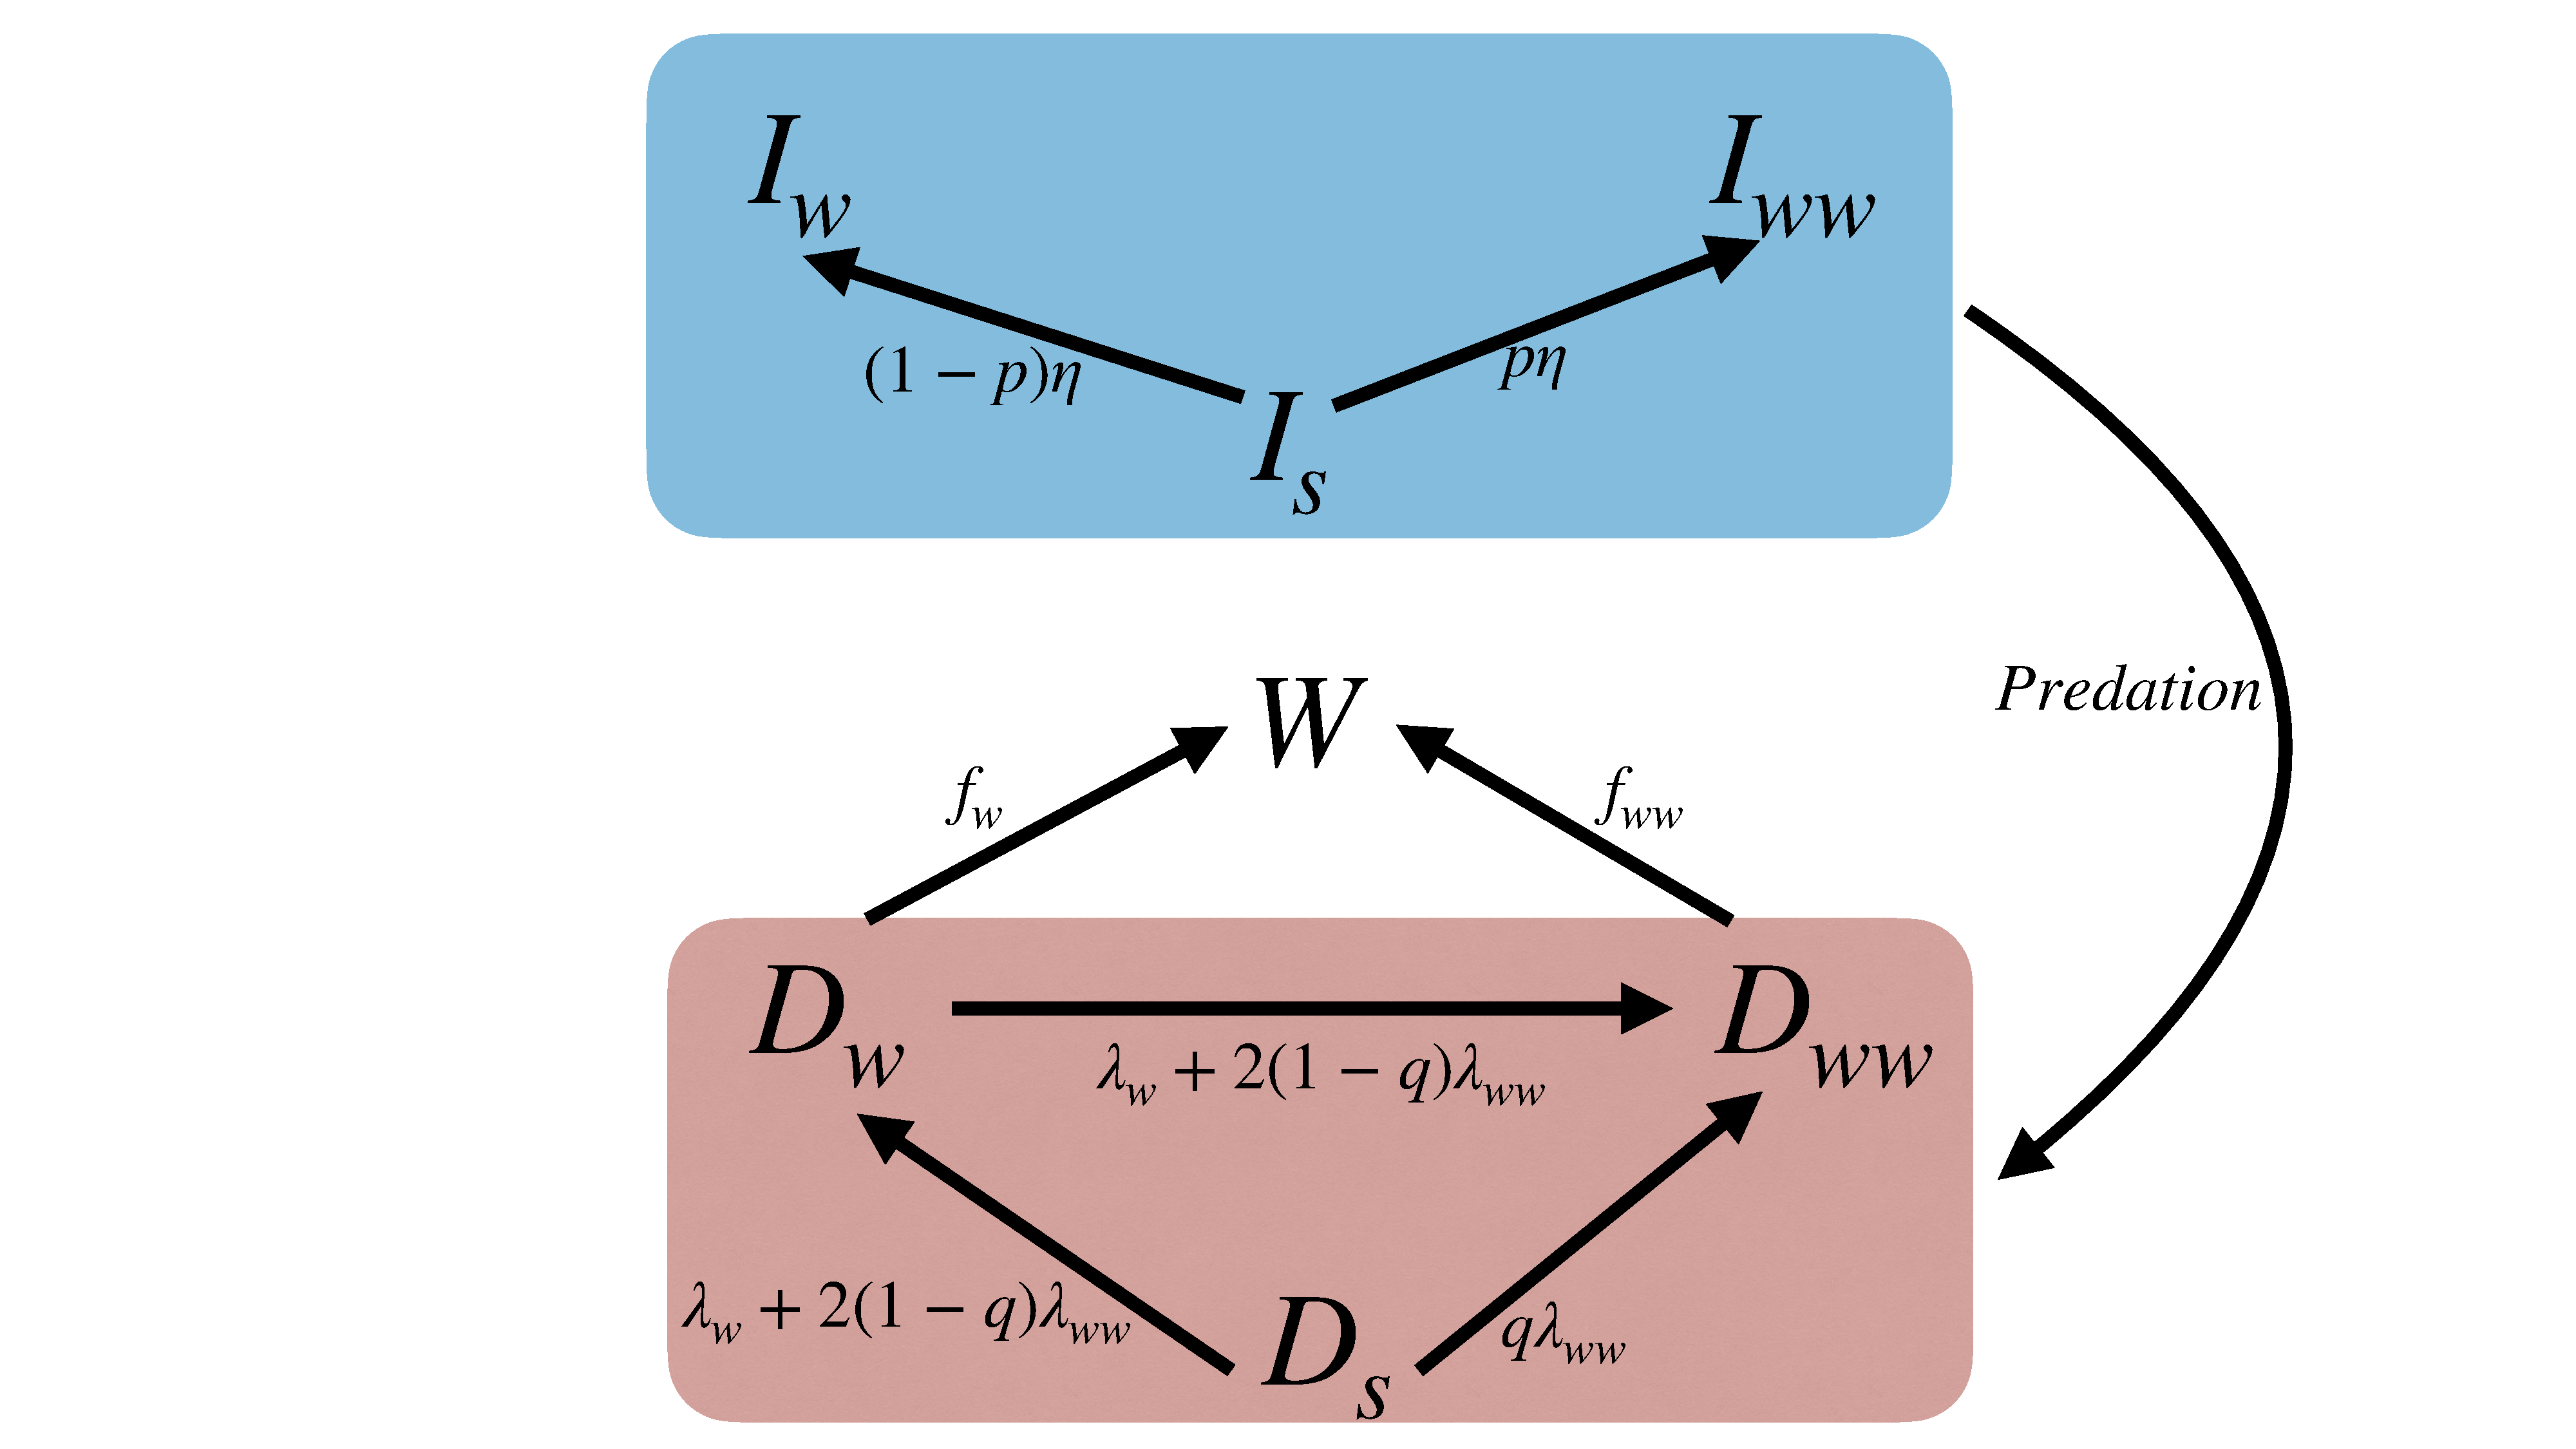
\includegraphics[width=\textwidth]{Figures/schematics.pdf}
\caption{Schematic of the model. The compartments of intermediate hosts are in the blue box, including $I_s$ (susceptible host), $I_w$ (singly infected host), and $I_{ww}$ (doubly infected host). The compartments of definitive hosts are in the red box, including $D_s$ (susceptible host), $D_w$ (singly infected host), and $D_{ww}$ (doubly infected host). Definitive hosts prey upon intermediate host and infection happens when infected intermediate hosts are eaten by definitive hosts. $W$ represents the parasite pool in the environment where parasites are released from the definitive hosts.}
\label{fig:schematic}
\end{figure}

\subsection*{Basic reproduction ratio $R_0$}

We calculate the basic reproduction ratio $R_0$ of the parasite using the next generation method (ref) (details are in supplementary).
\begin{align}
R_0 = & \gamma I_s^* \frac{ p q \beta_{ww}}{\alpha_{ww} + d + \Pi_{ww}} \frac{D_s^*}{\mu +\sigma_{ww}} \frac{f_{ww}}{\delta +\gamma I_s^*} + \nonumber \\
& \gamma  I_s^* \left( \frac{ (1-p)\beta_w}{\alpha_w + d + \Pi_w} + \frac{2 p (1-q) \beta_{ww}}{\alpha_{ww} + d + \Pi_{ww}} \right) \frac{D_s^*}{\lambda_w + 2 (1-q) \lambda_{ww}  + \mu + \sigma_w} \frac{f_w}{\delta +\gamma  I_s^*}
\end{align}

where $I_s^*$ and $D_s^*$ are the density of susceptible intermediate and definitive hosts at the disease free equilibrium. The expression of $R_0$ indicates the possible reproduction routes of a parasite when being introduced in a disease-free population. The routes can be via double infections or single infection. The first component corresponds to the double infections route, in which the focal parasite co-transmit with another parasite into a susceptible intermediate host, then co-transmit into a susceptible definitive host and reproduce. The second component corresponds to the single infection route, in which the focal parasite infects a susceptible intermediate host, either via singly or doubly infections. It then transmit alone into the susceptible definitive host, and eventually reproduce. The compartment with sequential infection do not appear in the reproduction route via double infections because parasites are assumed rare in a susceptible prey-predator population.


If $R_0 > 1$, a parasite can spread in the population. To further understand the effect of manipulation on the fitness of the parasites and the ecological dynamics of the system, we will specify the predation functions $P_s, P_w, P_{ww}$, and the birth functions $R$ and $B$ of respectively the intermediate and definitive host. For simplicity, we consider linear functions for predation 

\begin{align*}
& \P_s(D_s + D_w + D_{ww}) = \rho (D_s + D_w + D_{ww}) \\
& \P_w(D_s, D_w, D_{ww}, \beta_w) = (\rho + \beta_w) (D_s + D_w + D_{ww}) \\
& \P_{ww}(D_s, D_w, D_{ww}, \beta_{ww}) =  (\rho + \beta_{ww}) (D_s + D_w + D_{ww})
\end{align*}

where $\rho$ is the baseline capture rate of the predator on the prey. If an intermediate hosts is infected, it is captured by the definitive hosts with rate $\rho + \beta_w$ if it is singly infected, and with rate $\rho + \beta_{ww}$ if it is doubly infected. Zero values for $\beta_w$ and $\beta_{ww}$ suggest no manipulation. We consider a linear function of the birth of definitive hosts

\begin{align*}
B(D_s, D_w, D_{ww}, I_s, I_w, I_{ww}) = \rho c (D_s + D_w + D_{ww}) (I_s + I_w + I_{ww})
\end{align*}

where c is the efficiency of converting preys into offspring. It is noted that the birth rate of the predators depend on the capture rate but, to our best knowledge, there are no evident that host manipulation affects the birth rate of the predators.

\subsection*{Linear birth function of intermediate hosts}
We consider the system when the birth function $R$ of the intermediate host is linear, specifically, $R(I_s, I_w, I_ww) = r(I_s + I_w + I_ww)$. The equilibrium of intermediate and definitive hosts in the disease-free state are

\begin{align*}
& I_{s0}^* = \frac{\mu}{c \rho} \\
& D_{s0}^* = \frac{r - d}{\rho}
\end{align*}

This equilibrium is always unstable. 
We always observe cyclic behaviour of the equilibrium because, at this equilibrium, the jacobian matrix of the system (\ref{odes:ihosts}, \ref{odes:dhosts}, \ref{odes:eparasite}) always has one imaginary eigenvalue with a positive real part. 
This follows from the Lotka-Voltera system using linear functions for prey birth and predation (reference...). 
Because the disease-free dynamics is cyclic, it is difficult to analyse the spread of a parasite (often evaluated when the disease-free state is stable). 
Here, even if we solve the inequality $R_0 > 1$, which happens when the transmission rate from the environment to intermediate hosts $\gamma$ is greater than a threshold (the expression of the threshold is too complicated, hence it is not useful to write it here). 
In addition, the reproduction of the parasites has to be sufficiently large (again, the expression of the thresholds are too complicated such that it is useless to write it here).

Our simulations show that the parasite cannot persist even when its reproduction ratio is greater than one (Figure \ref{fig:diseasefree:linear}). This result is, however, in agreement with the conclusion in \citet{Ripa:Evol:2013}, which suggests that it is harder for a mutant to invade a cyclic population. 
In our case, it is not the invasion of a mutant but a specific parasite in a cyclic disease-free host population. 
This issue deserves a more thorough investigation. 
To obtain a stable disease circulation state, we use a non-linear birth function of intermediate hosts. The following sections focus on analysing the ecological dynamics of the complex lifecycle parasite under different scenario of its manipulative ability.

\begin{figure}
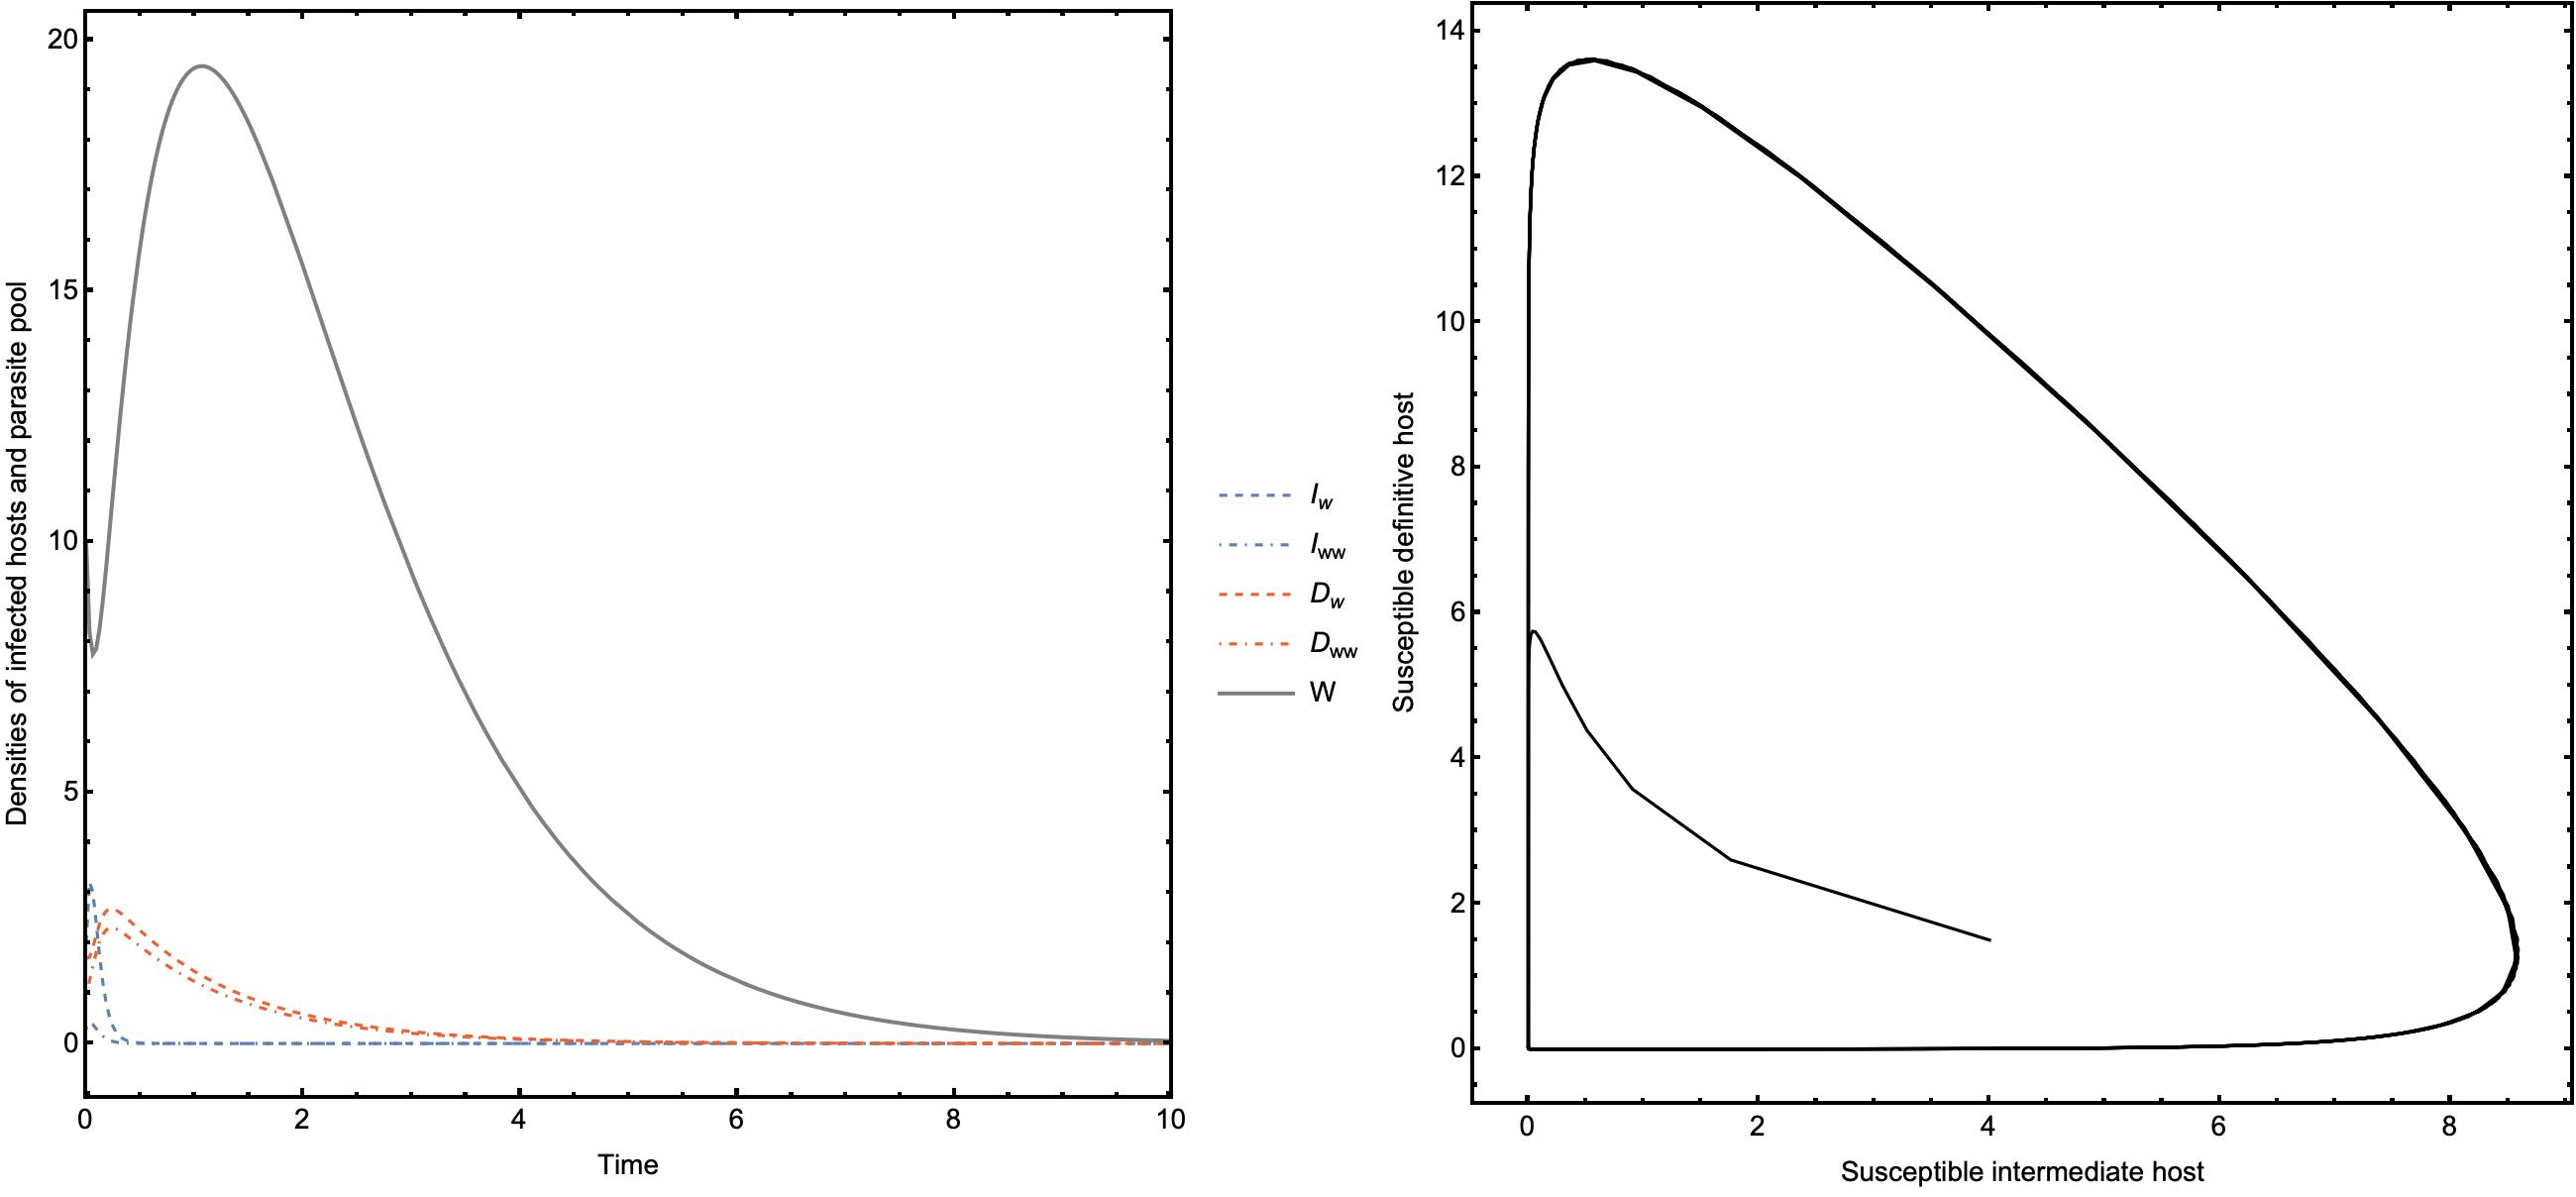
\includegraphics[width=\textwidth]{Figures/diseasefree_linear.jpg}
\caption{Disease-free equilibrium using linear birth function. Solid gray line indicate the density of free-living parasites, blue lines indicate infected intermediate hosts while red lines indicate infected definitive hosts. Dashed lines indicate singly infected hosts while dot-dashed lines indicate doubly infected hosts. Parameter values  $\rho = 1.2, \  d = 0.9, \  r = 2.5, \ \gamma = 2.9, \ \alpha_w =  \alpha_{ww} =  0, \ \beta_w  = 1.5, \ \beta_{ww} = 1.5, \ p = 0.1,  \ c = 1.4, \ \mu = 0.9,  \ \sigma_w = \sigma_{ww} = 0, \ q = 0.01, \  f_w = 6.5, \  f_{ww} = 7.5, \ \delta = 0.9$ } 
\label{fig:diseasefree:linear}
\end{figure}

\subsection*{Non-linear birth function of intermediate hosts}
The non-linear birth function of intermediate hosts is as followed

\begin{align*}
R(I_w, I_s,I_{ww}) = r (I_s + I_w + I_{ww}) (1 - k (I_s + I_w + I_{ww}))
\end{align*}

where $k$ is the intraspecific competition coefficient. The disease-free equilibrium is as follows

\begin{align*}
& I_s = \frac{\mu}{c \rho } \\
& D_s = \frac{c \rho  (r-d) - k \mu  r}{c \rho ^2}
\end{align*}

This equilibrium is stable if,

\begin{align*}
& r > d \\
& \frac{2 c \rho  \left(\sqrt{\frac{-d+\mu +r}{\mu }}-1\right)}{r}\leq k < \frac{c \rho  (r-d)}{\mu  r} \\
& \mu >\frac{4 c^2 \rho ^2 r - 4 c^2 d \rho ^2}{4 c k \rho r + k^2 r^2}
\end{align*}

The above conditions suggest that the intrinsic reproduction of intermediate hosts $r$ needs to be greater than their natural mortality rate $d$. 
More importantly, the intraspecific competition coefficient has to be within a range. 
It is neither too small such that the population cannot grow to infinity nor too large such that the population cannot survive. 
Finally, the natural mortality rate of the definitive host has to be sufficiently large. Satisfying such conditions, we obtain a stable disease-free equilibrium (Figure \ref{fig:ecotraject:nonlinear}).

\begin{figure}[!ht]
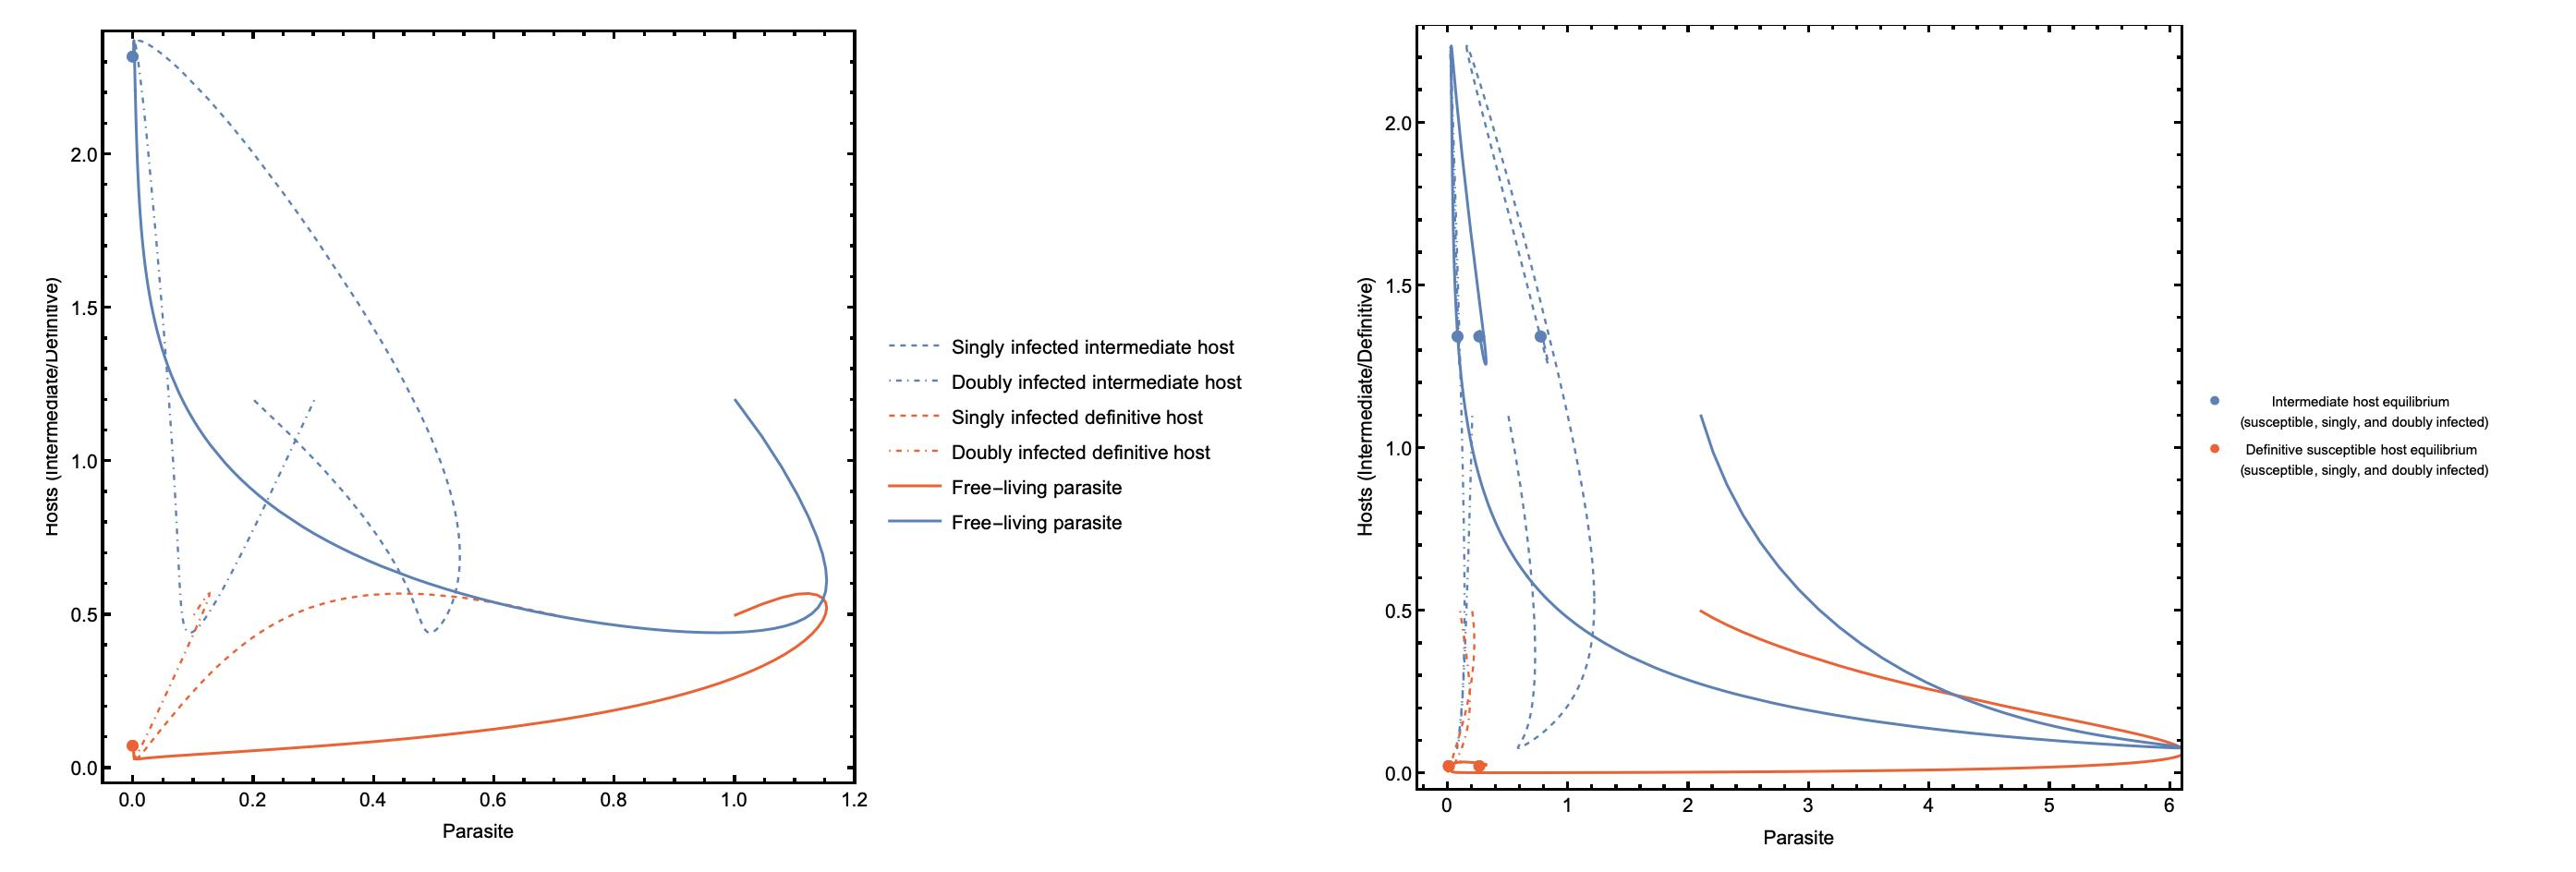
\includegraphics[width=\textwidth]{Figures/ecotraject_nonlinear.jpeg}
\caption{A) Trajectories of parasite and host dynamics. The host includes both intermediate (blue) and definitive (orange) ones. A) Disease free equilibrium where parasite densities is zero. B) Disease stable equilibrium where there are multiple parasite densities which correspond to free parasite pool, singly infected hosts and doubly infected hosts. Parameters for disease free equilibrium $\rho =  1.2, \ d = 0.9, \  r = 2.5, \ \gamma =  2.9, \alpha_w = \alpha_{ww} =  0, \ \beta_w = \beta_{ww} = 1.5, \ p = 0.1, \  c = 1.4, \ \mu = 3.9, \ \sigma_w = \sigma_{ww} = 0, \ q = 0.01, \ f_w = f_{ww} = 7.5, \ \delta = 0.9, \ k = 0.26$. Disease stable equilibrium have the same parameter values except for higher host manipulation $ \beta_w =  \beta_{ww} = 4.5$ and parasite reproduction $ f_w  = f_{ww} = 45$}
\label{fig:ecotraject:nonlinear}
\end{figure}

When a parasite is introduced in the disease-free equilibrium, it can spread if its reproduction ratio $R_0 > 1$. 
Since the expression is complicated, we could not obtain solutions for this inequality without assumptions. 
Assuming that double infections and single infection result in the same parasite virulence and parasite reproduction, that is, $\alpha_w = \alpha_{ww}$, $\sigma_w = \sigma_{ww}$,and $f_w = \epsilon f_{ww}$, we found the the parasite can establish and spread in the population of intermediate and definitive hosts if its reproduction value in single infection $f_w$ is greater than a threshold (the expression of the threshold is rather complicated, therefore it is not useful to write down its expression) (Figure \ref{fig:bistability}). It should be noted that parasite reproduction is extremely large compared to other parameters (its value is 40 times greater than the values of other parameters), suggesting that trophically transmitted parasites have to release a large amount of offspring into the environment to maintain its persistence. Interestingly, if the reproduction rate of the parasite in double infection state is greater than that in single infection state, bistability can occur such that the parasite population will crash if it is disturbed and become too small (Figure \ref{fig:bistability}A, B). In that case, as parasite reproduction increases, the density of singly infected definitive host saturated instead of increasing as in the case when there is no difference in reproduction between singly and doubly infection. 

\begin{figure}[!ht]
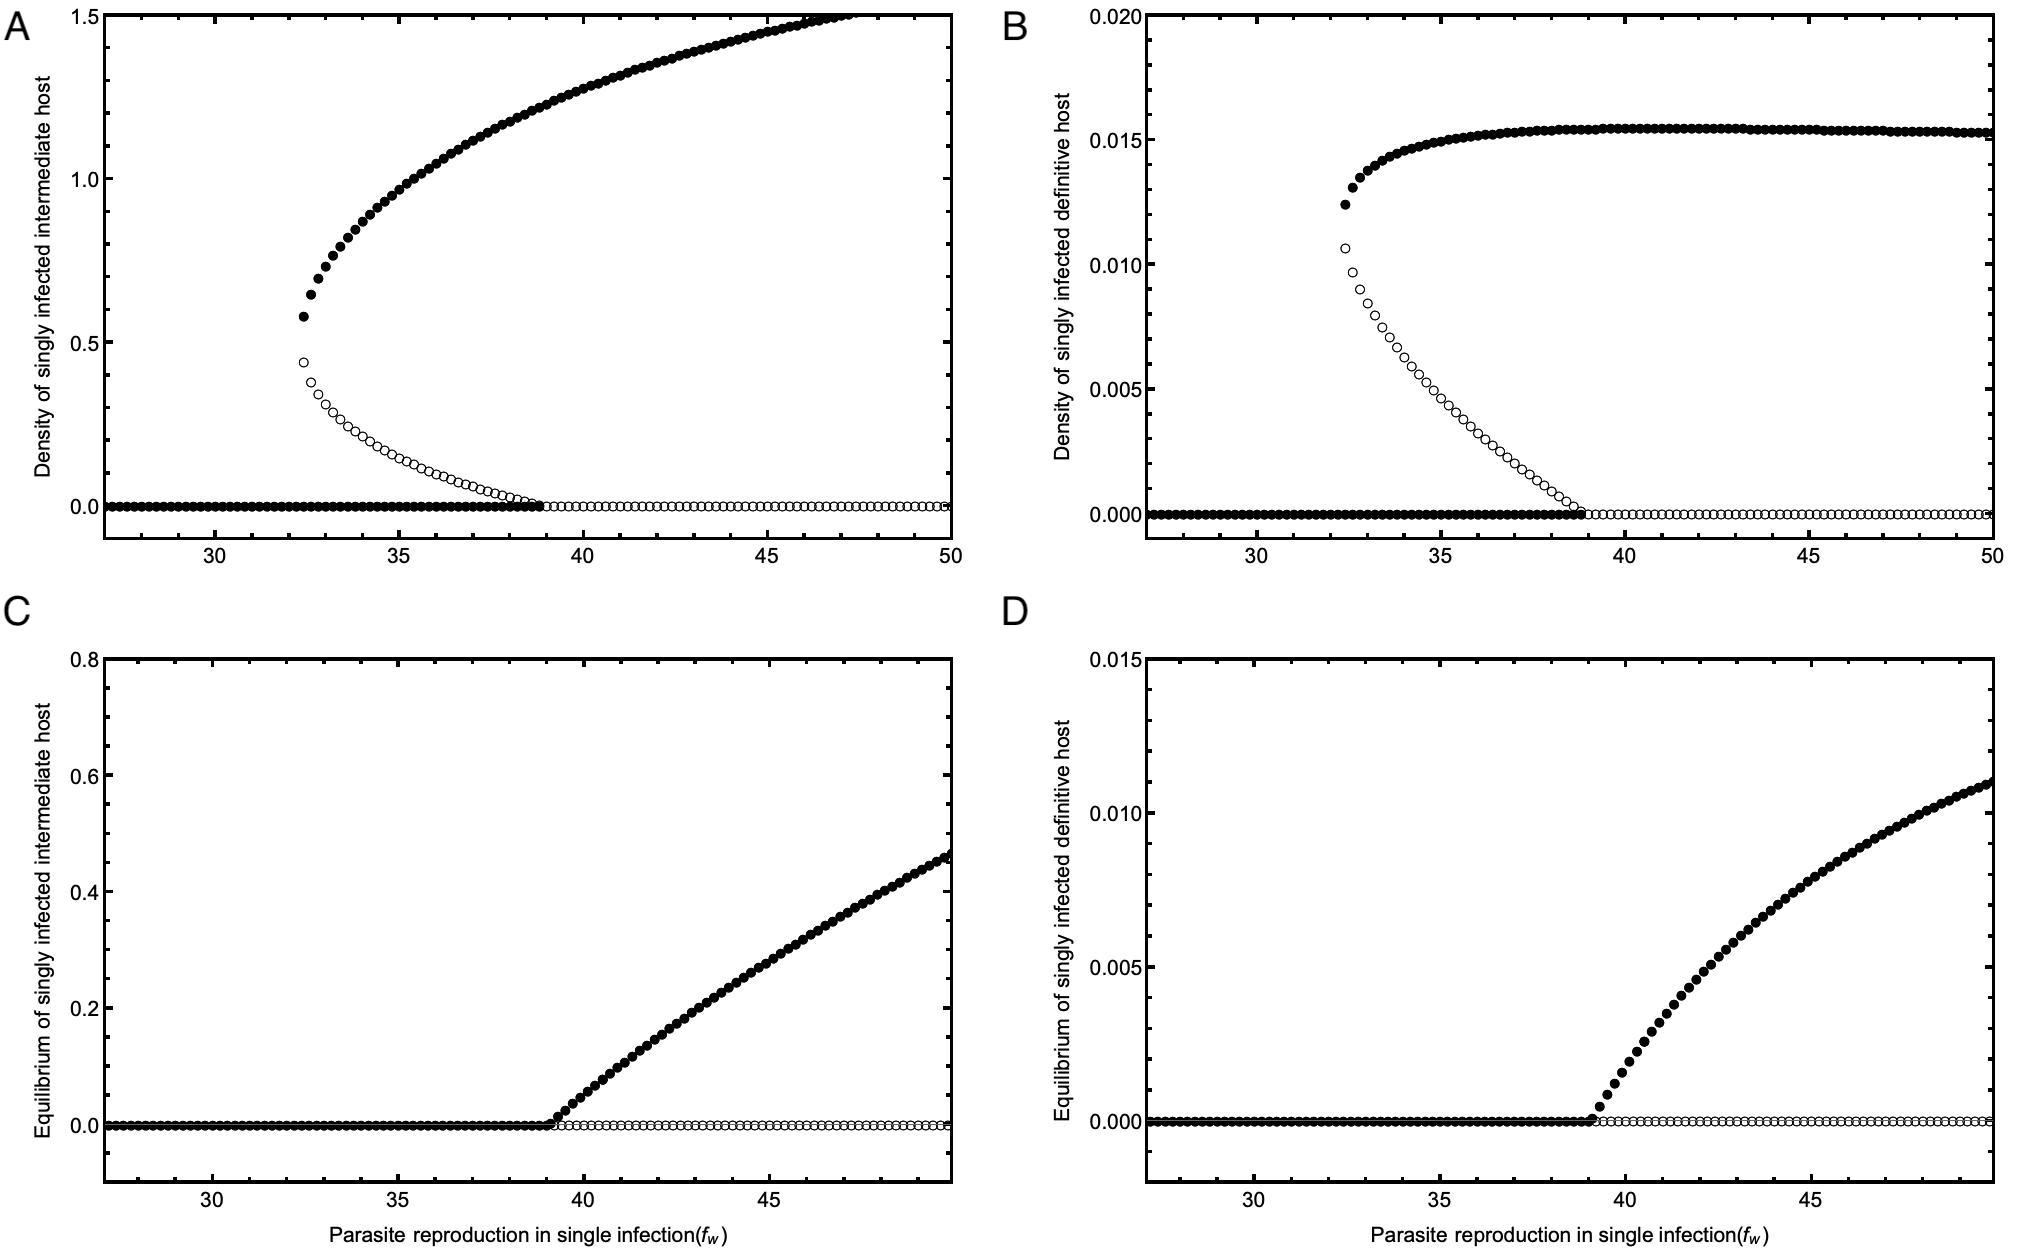
\includegraphics[width = \textwidth]{Figures/bistability.jpeg}
\caption{Effect of parasite reproduction on the ecological dynamics. A, B) When reproduction of parasites in singly infected hosts is four times greater than those in doubly infected hosts $\epsilon = 4$. C, D) When reproduction of parasites are the same in singly and doubly infected hosts $\epsilon = 1$. Filled circles indicate stable equilibrium and open circles indicate unstable equilibrium. Parameter $\rho = 1.2, \  d = 0.9, \  r = 2.5, \ \gamma = 2.9, \ \alpha_w = 0, \ \alpha_ww =  0, \ \beta_w = 1.5, \ \beta_{ww} = 1.5, \ p = 0.1, \  c = 1.4, \ \mu = 3.9,  \ \sigma_w = 0, \ \sigma_{ww} = 0, \  q = 0.01, \ \delta = 0.9, \ k = 0.26$
}
\label{fig:bistability}
\end{figure}

\subsection*{The effect of host manipulation on ecological dynamics}


Cooperation in parasite manipulation increases the basic reproduction ratio of the parasite. However, if the ability to manipulate host in single infection is not sufficiently strong, such cooperation widen the bistable state of the system (Figure \ref{fig:manipR0}). Within the area of bistability, the basic reproduction ratio is less than one, suggesting that parasites that are highly cooperative in manipulation in double infection yet have low ability to manipulate when alone cannot spread in a disease free prey-predator (or intermediate/definitive host) population. 

\begin{figure}
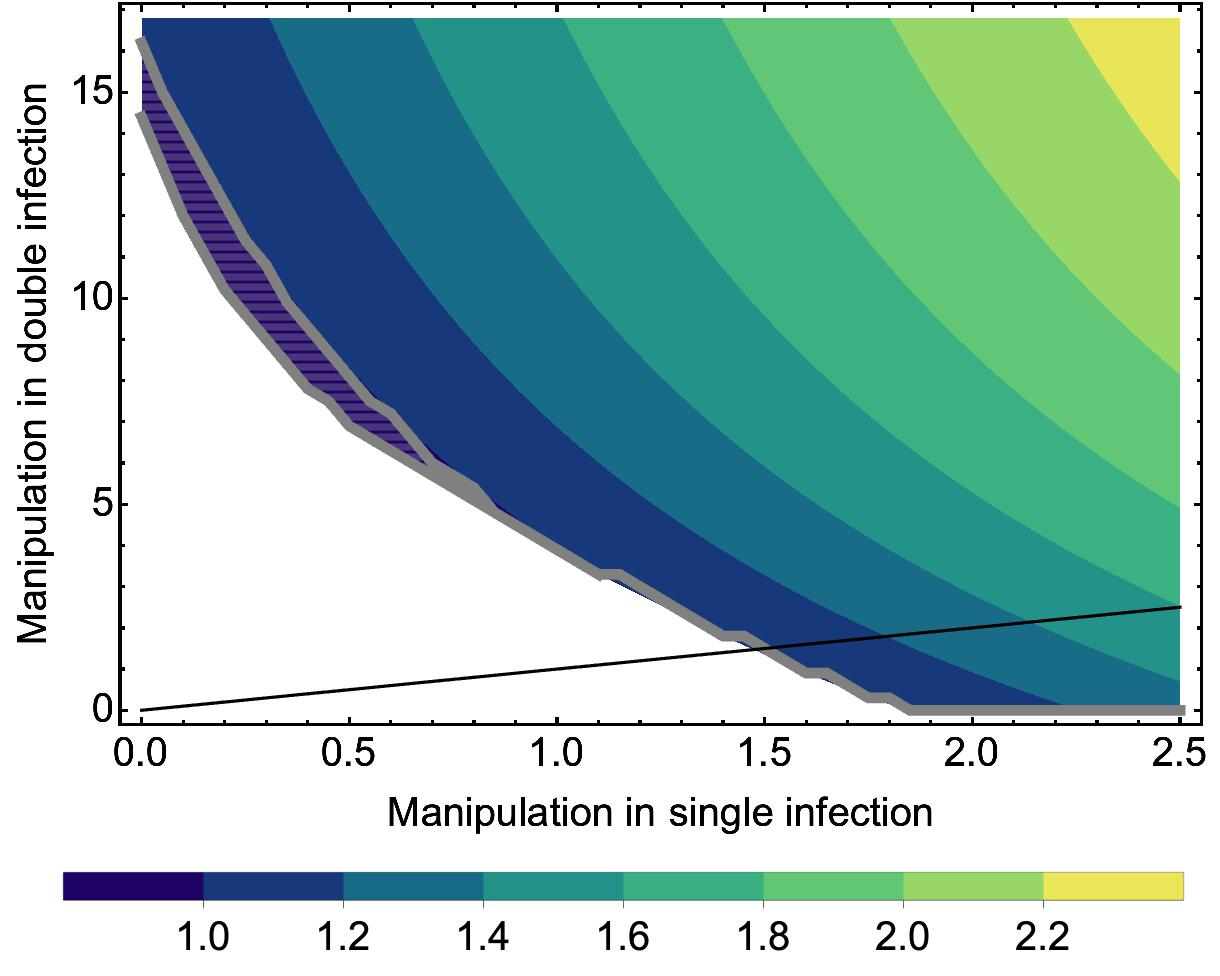
\includegraphics[width=\textwidth]{Figures/manip_bifur_R0.jpeg}
\caption{A). Bistability region when cooperation in manipulation is high (dark green area). As manipulation in single infection increases, the system only has one stable equilibiria (light green area). On the black line, manipulation is indifference between single infection and double infection. B) Basic reproduction ratio $R_0$ with respect to manipulation in single and double infection. $R_0 < 1$ indicates that the parasite cannot establish in a disease free prey-predator population.}
\label{fig:manipR0}
\end{figure}

Parasites can be also cooperative in reproduction, that is, parasites in doubly infected definitive hosts have higher reproduction rate than parasites in singly infected definitive hosts. Without any assumption on the relationship between manipulative ability and reproduction, parasites can be cooperative in both manipulation and reproduction. Interestingly, the higher the cooperation in manipulation and reproduction, the larger the area of bistability (Figure \ref{fig:manipbifur}). This suggests that systems, in which parasites have much higher manipulative ability and reproduction rate when coinfected than when singly infected, are more unstable than systems with parasites that are less cooperative, or systems with parasites that sabotage each other in coinfection. \cite{akbari:ACSSynBio:2014}

\begin{figure}[!ht]
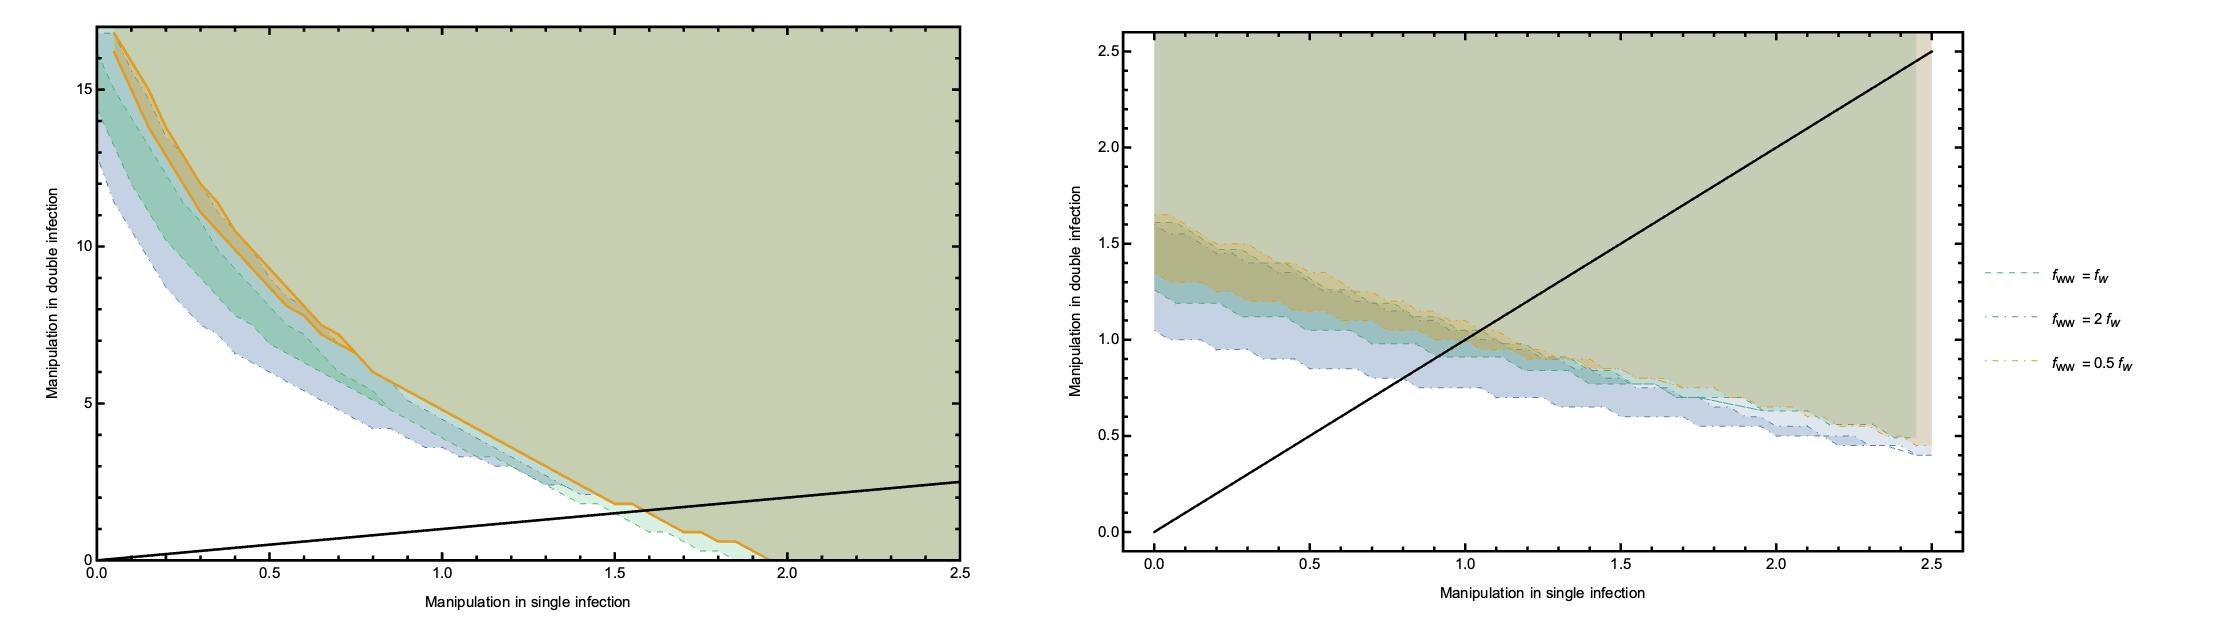
\includegraphics[width=\textwidth]{Figures/manip_bifurcation.jpeg}
\caption{Bifurcation graph of $\beta_w$ (manipulation in singly infected host) and $\beta_{ww}$ (manipulation in doubly infected host) when cotransmission from the parasite pool to intermediate host is small $p = 0.01$ (A) and big $p = 0.5$. The white area is where the parasite goes extinct. Bistability occurs in the bounded areas. Manipulation is indifference between single infection and double infection on the black thick line. Common parameter:  $\rho = 1.2, \ d = 0.9, \ r = 2.5, \ \gamma = 2.9, \ \alpha_w = 0, \ \alpha_{ww} = 0, \ p = 0.1, \ c = 1.4, \ \mu = 3.9, \ \sigma_w = 0, \ \sigma_ww = 0, \ q = 0.01, \ \delta = 0.9, \ k = 0.26, \ \epsilon = 0.5$. Orange thick boundary indicates when reproduction of double infection is smaller than that of single infection ($\epsilon = 0.5, f_w = 36$), B) Dashed green boundary indicates when there is no difference in reproduction between single infection and double infection ($\epsilon = 1, f_w = 36$), C) Dot-dashed blue boundary indicates when reproduction in double infection is greater than that of single infection ($\epsilon = 2, f_w = 35$).}
\label{fig:manipbifur}
\end{figure}


\section*{Discussion}


\section*{Conclusion}


%%%%%%%%%%%%%%%%%%%%%
% Acknowledgments
%%%%%%%%%%%%%%%%%%%%%
% You may wish to remove the Acknowledgments section while your paper 
% is under review (unless you wish to waive your anonymity under
% double-blind review) if the Acknowledgments reveal your identity.
% If you remove this section, you will need to add it back in to your
% final files after acceptance.

 \section*{Acknowledgments}


 \section*{Statement of Authorship}
 
\section*{Data and Code Availability}
All data and simulation codes for generating figures are available on 

%All data and simulation codes for generating figures are available on \href{https://anonymous.4open.science/r/genedrives_mating-6841/}{Github}   
%(\url{https://anonymous.4open.science/r/genedrives_mating-6841/}).


\newpage{}

%% Reseting the counters for equations, figures, tables
\renewcommand{\theequation}{A\arabic{equation}}
% redefine the command that creates the equation number.
\renewcommand{\thetable}{A\arabic{table}}
\renewcommand{\thefigure}{A\arabic{figure}}

\setcounter{figure}{0}
\setcounter{equation}{0}  % reset counter 
\setcounter{table}{0}

\section*{Appendix A}


\section*{Appendix B}


\newpage{}

%%%%%%%%%%%%%%%%%%%%%
% Bibliography
%%%%%%%%%%%%%%%%%%%%%
% You can either type your references following the examples below, or
% compile your BiBTeX database and paste the contents of your .bbl file
% here. The amnatnat.bst style file should work for this---but please
% let us know if you run into any hitches with it!
%
% If you upload a .bib file with your submission, please upload the .bbl
% file as well; this will be required for typesetting.
%
% The list below includes sample journal articles, book chapters, and
% Dryad references.

\bibliographystyle{amnatnat}
%\bibliography{\string~/Bibtex/et.bib}

\begin{thebibliography}{24}
\providecommand{\natexlab}[1]{#1}

\bibitem[{Alizon (2012)}]{Alizon2012}
Samuel Alizon. 2012.
\newblock Parasite co-transmission and the evolutionary epidemiology of
  virulence.
\newblock {\em Evolution}, 67(4):921--933, November 2012.

\bibitem[{Alizon et~al.(2013)Alizon, de~Roode, Michalakis}]{Alizon2013}
Samuel Alizon, Jacobus~C. de~Roode, and Yannis Michalakis. 2013.
\newblock Multiple infections and the evolution of virulence.
\newblock {\em Ecology Letters}, 16(4):556--567, January 2013.

\bibitem[{Alizon and van Baalen(2008)}]{Alizon2008}
Samuel Alizon and Minus van Baalen. 2008.
\newblock Multiple infections, immune dynamics, and the evolution of virulence.
\newblock {\em The American Naturalist}, 172(4):E150--E168, October 2008.

\bibitem[{Benesh(2016)}]{Benesh:2016dj}
Daniel~P Benesh. 2016.
\newblock {Autonomy and integration in complex parasite life cycles.}
\newblock {\em Parasitology}, 143(14):1824 -- 1846, 2016.

\bibitem[{Choisy and de~Roode(2010)}]{Choisy2010}
Marc Choisy and Jacobus~C. de~Roode. 2010.
\newblock Mixed infections and the evolution of virulence: Effects of resource
  competition, parasite plasticity, and impaired host immunity.
\newblock {\em The American Naturalist}, 175(5):E105--E118, May 2010.

\bibitem[{Fenton and Rands(2006)}]{Fenton2006}
A.~Fenton and S.~A. Rands. 2006.
\newblock The impact of parasite manipulation and predator foraging behavior on
  predator - prey communitites.
\newblock {\em Ecology}, 87(11):2832--2841, November 2006.

\bibitem[{Gandon(2018)}]{Gandon2018}
Sylvain Gandon. 2018.
\newblock Evolution and manipulation of vector host choice.
\newblock {\em The American Naturalist}, 192(1):23--34, July 2018.

\bibitem[{Hadeler and Freedman(1989)}]{Hadeler1989}
K.~P. Hadeler and H.~I. Freedman. 1989.
\newblock Predator-prey populations with parasitic infection.
\newblock {\em Journal of Mathematical Biology}, 27(6):609--631, November 1989.

\bibitem[{Hafer and Milinski(2015)}]{Hafer:2015gl}
Nina Hafer and Manfred Milinski. 2015.
\newblock {When parasites disagree: evidence for parasite-induced sabotage of
  host manipulation.}
\newblock {\em Evolution}, 69(3):611 -- 620, 2015.

\bibitem[{Hosack et~al.(2008)Hosack, Rossignol, and van~den Driessche}]{Hosack2008}
Geoffrey~R. Hosack, Philippe~A. Rossignol, and P.~van~den Driessche. 2008.
\newblock The control of vector-borne disease epidemics.
\newblock {\em Journal of Theoretical Biology}, 255(1):16--25, November 2008.

\bibitem[{Hughes(2012)}]{Hughes2012}
David~P Hughes, Jacques Brodeur, and Frederic Thomas. 2012.
\newblock {\em Host Manipulation by Parasites}.
\newblock Oxford University Press, London, England, June 2012.

\bibitem[{Iritani and Sato(2018)}]{Iritani2018}
Ryosuke Iritani and Takuya Sato. 2018.
\newblock Host-manipulation by trophically transmitted parasites: The
  switcher-paradigm.
\newblock {\em Trends in Parasitology}, 34(11):934--944, November 2018.

\bibitem[{Molyneux and Jefferies(1986)}]{molyneux_jefferies1986}
D.~H. Molyneux and D.~Jefferies. 1986.
\newblock Feeding behaviour of pathogen-infected vectors.
\newblock {\em Parasitology}, 92(3):721–736, 1986.

\bibitem[{Parker et~al.(2003)Parker, Chubb, Roberts, Michaud, and Milinski}]{Parker2003}
G.~A. Parker, J.~C. Chubb, G.~N. Roberts, M.~Michaud, and M.~Milinski. 2003.
\newblock Optimal growth strategies of larval helminths in their intermediate
  hosts.
\newblock {\em Journal of Evolutionary Biology}, 16(1):47--54, January 2003.

\bibitem[{Ripa and Dieckmann(2013)}]{Ripa:Evol:2013}
Jörgen Ripa and Ulf Dieckmann. 2013.
\newblock Mutant invasions and adaptive dynamics in variable environments.
\newblock {\em Evolution}, 67(5):1279--1290, 2013.

\bibitem[{Rogawa et~al.(2018)Rogawa, Ogata, and Mougi}]{Rogawa2018}
Akiyoshi Rogawa, Shigeki Ogata, and Akihiko Mougi. 2018.
\newblock Parasite transmission between trophic levels stabilizes
  predator{\textendash}prey interaction.
\newblock {\em Scientific Reports}, 8(1), August 2018.

\bibitem[{Roger and Bates(2007)}]{Rogers2007}
Matthew~E Rogers and Paul~A Bates. 2007.
\newblock Leishmania manipulation of sand fly feeding behavior results in
  enhanced transmission.
\newblock {\em {PLoS} Pathogens}, 3(6):e91, 2007.

\bibitem[{Roosien et~al.(2013)Roosien, Gomulkiewicz, Ingwell, Bosque-Perez, Rajabaskar, and Eigenbrode}]{Roosien2013}
Bryan~K. Roosien, Richard Gomulkiewicz, Laura~L. Ingwell, Nilsa~A. 2013.
  Bosque-P{\'{e}}rez, Dheivasigamani Rajabaskar, and Sanford~D. Eigenbrode.
\newblock Conditional vector preference aids the spread of plant pathogens:
  Results from a model.
\newblock {\em Environmental Entomology}, 42(6):1299--1308, December 2013.

\bibitem[{Seppala and Jokela(2008)}]{Seppl2008}
Otto Seppala and Jukka Jokela. 2008.
\newblock Host manipulation as a parasite transmission strategy when
  manipulation is exploited by non-host predators.
\newblock {\em Biology Letters}, 4(6):663--666, August 2008.

\bibitem[{van Baalen and Sabelis(1995)}]{vanBaalen1995}
Minus van Baalen and Maurice~W. Sabelis. 1995.
\newblock The dynamics of multiple infection and the evolution of virulence.
\newblock {\em The American Naturalist}, 146(6):881--910, December 1995.

\bibitem[Vickery and Poulin(2009)]{Vickery2009}
William~L. Vickery and Robert Poulin. 2009.
\newblock The evolution of host manipulation by parasites: a game theory
  analysis.
\newblock {\em Evolutionary Ecology}, 24(4):773--788, November 2009.

\bibitem[Wedekind and Milinski(1996)]{Wedekind1996}
C.~Wedekind and M.~Milinski. 1996.
\newblock Do three-spined sticklebacks avoid consuming copepods, the first
  intermediate host of \textit{Schistocephalus solidus}? - an experimental
  analysis of behavioural resistance.
\newblock {\em Parasitology}, 112(4):371--383, April 1996.

\bibitem[{Zimmer(2001)}]{zimmer:book:2001}
Carl Zimmer. 2001.
\newblock {\em {Parasite Rex: Inside the Bizarre World of Nature's Most
  Dangerous Creatures}}.
\newblock Atria Books, 2001.

\end{thebibliography}

\newpage{}

\section*{Tables}
\renewcommand{\thetable}{\arabic{table}}
\setcounter{table}{0}

\begin{table}[h]
%\caption{Examples of natural drive elements with properties simulated in this study.}
%\label{Table:Driveelements}
%\centering
%\begin{tabular}{lllll}\hline
%Species & Drive element & Drive type \& parameters & Ecological properties
% \\ \hline
%\textit{Tribolium castaneum}  & Medea & Viability drive $d$ & Probably low k, highly \\
%  & & & polyandrous\\
 %   & & & \citep{pai:EntoEA:2020} \\
%\textit{Drosophila melanogaster}  & Selfish Segregation  & Distortion drive
%$p$,$c$ & Probably low k, Polyandry \\ 
%& Distorter (SD) & & with some re-mating \\
%& & & latency \citep{singh:CurrSci:2004}\\
%\textit{Mus musculus}  & t-haplotype & Distortion drive
%$p$,$c$ & Probably low k, \\ 
%& & & Polyandry ($r=2,$, \\ 
%& & & \citep{birand:MolEcol:2022}) \\ \hline 
%\end{tabular}
%\bigskip{}
%\\
%{\footnotesize Note: Table titles should be short. Further details should go in a `notes' area after the tabular environment, like this. $^a$ Published the first description of \textit{Dimetrodon}.}
\end{table}
%
\newpage{}

\section*{Figure legends}

\renewcommand{\thefigure}{\arabic{figure}}
\setcounter{figure}{0}
%%

%\begin{figure}[h!]
 %   \centering
% \includegraphics[width=0.65\columnwidth]{figure1.eps}
 %   \caption{\textbf{Pictorial representation of the three mating complexities: mate-choice, mating network, and mating system that can affect gene drive's population dynamics.}}
%    \label{fig:fig1}    
%\end{figure}
%%


% \subsection*{figure legends for Appendices}

\renewcommand{\thefigure}{A\arabic{figure}}
\setcounter{figure}{0}


\end{document}
